\section{Quadratic: degree=2}
\label{sec.quadratic}

\subsection{Objectives}
The assignment in this section is:
\begin{enumerate}
\item Complete the file \code{src/quadratic.py} by writing a Python
  function which computes and returns the x-intercepts of a parabola whose
  equation is \[y=a x^2 + b x + c\,.\]
\item    You'll need to replace all occurrences of \code{raise NotImplementedError()}
  with correct python code which passes the tests.

\item Test the function in GitHub Code-Spaces by running the file\\
  \code{test/test\_quadratic.py}.
\end{enumerate}

\subsection{Overview}

\begin{figure}
\centering
%% derived from https://tex.stackexchange.com/questions/357538/graph-of-a-parabola-on-pgfplots
%% Thanks to Stefan Pinnow
%%     https://tex.stackexchange.com/users/95441/stefan-pinnow

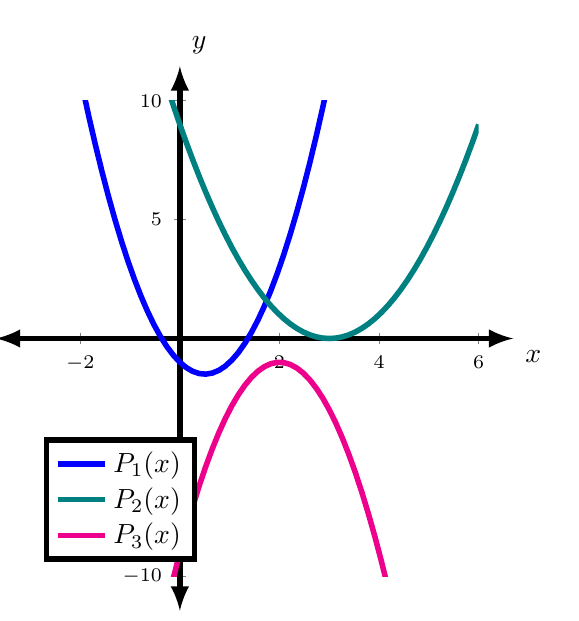
\begin{tikzpicture}
  \begin{axis}[
      legend pos=south west,
      width=.6\textwidth,
      height=3in,
      axis lines=middle,
      xmin=-3,
      xmax=6,
      ymin=-10,
      ymax=10,
      scaled ticks=false,
      line width=2pt,
      ticklabel style={font=\scriptsize},
      xlabel=$x$,
      ylabel=$y$,
      samples=70,
      domain=-3:6,
      axis line style={
        latex-latex,
        shorten >=-12.5pt,
        shorten <=-12.5pt,
      },
      xlabel style={at={(ticklabel* cs:1)}, xshift=12.5pt, anchor=north west},
      ylabel style={at={(ticklabel* cs:1)}, yshift=12.5pt, anchor=south west},
    ]
    
    \addplot[color=blue] {2*x^2 - 2*x - 1}; % 2 roots
    \addlegendentry{\(P_1(x)\)}
    \addplot[color=teal] {x^2 - 6*x + 9}; % 1 root
    \addlegendentry{\(P_2(x)\)}
    \addplot[color=magenta] {-2*x^2 + 8*x - 9}; % 0 roots
    \addlegendentry{\(P_3(x)\)}
  \end{axis}
\end{tikzpicture}
%

\caption{Parabolas}
\label{fig.parabola}
\end{figure}

A quadratic polynomial is of the form $P(x)=a x^2 + b x + c$.  If
$a=0$, then $P(x)$ is actually a first degree polynomial which can be
solved using the techniques described in Section~\ref{sec.line};
otherwise we need a more elaborate technique which is explained here in
Section~\ref{sec.quadratic}

We have the plots of three quadratic polynomials, $P_1(x)$, $P_2(x)$,
and $P_3(x)$, shown in Figure~\ref{fig.parabola}.  Each plot takes the
geometric form of a parabola.  As can be seen in the figure, the
parabola might intersect the x-axis twice (\eg, $P_1(x)$), once (\eg,
$P_2(x)$, or not at all (\eg, $P_3(x)$).

\begin{align*}
  P_1(x) &= 2x^2 - 2 x - 1\\
  P_2(x) &= x^2 -x + \frac{1}{4}\\
  P_3(x) &=  -2x^2 + 2x -2
\end{align*}


\subsection{The Math / The Theoretical}

To determine how many times a parabola touches the x-axis, we need to
find the roots of the corresponding quadratic (degree~2) polynomial of
the form $a x^2 + b x + c$.  The formula is called the \emph{quadratic
formula}:

\[x = \frac{-b\pm\sqrt{b^2 - 4a c}}{2a}\]

In particular,
we need to look at the expression under the square root, called the
discriminant: $b^2 - 4a c$.
\begin{itemize}
\item If the discriminant is positive, then the polynomial has two
  distinct real roots.
\item If the discriminant is zero, then the positive and negative
  square roots $\pm\sqrt{b^2 - 4a c}$ in the quadratic formula are
  both 0; thus the polynomial has 1 single root where the parabola
  touches the x-axes tangentially.
  
\item If the discriminant is negative, then there is a negative under
  the radical sign; thus the polynomial has no real roots.  The
  polynomial does have complex roots; however we will ignore complex
  roots for this atelier.
\end{itemize}

\subsection{The Programming / The Practical}

Steps for computing roots of a polynomial of degree~2.
\begin{enumerate}
\item Assume the coefficients of $P(x)$ are in the variables \code{a},
  \code{b}, and \code{c}.
\item If \code{a == 0}, then delegate to previous solution by calling
  the function \code{find\_x\_intercept} and returning its value.
  Note that \\ \code{find\_x\_intercept} takes two arguments, which it
  calls \code{a} and \code{b}, but these are not \code{a} and \code{b}
  of the quadratic.  In fact for \code{find\_x\_intercept}, \code{a}
  is the coefficients of $x$ and \code{b} is the bias term of $a x +
  b$.  However, for the quadratic, \code{a} is the coefficient of
  $x^2$, and \code{b} is the code of $x$ in $a x^2 + b x + c$.
\item Compute the discriminant, storing in the variable
  \code{discriminant}.
\item Test three conditions.
  \begin{enumerate}
  \item If the discriminant is positive, then return a list of the two
    roots.
  \item If the discriminant is zero (or very close to zero), then
    return a list (of length two) of the same root twice.
  \item If the discriminant is negative ( $< -\varepsilon$), then
    return an empty list~\code{[]}.
  \end{enumerate}

\item Test your code by running the pre-defined tests in
  \\ \code{tests/test\_quadratic.py}.

\item Look at the proposed solution in \code{solutions/quadratic.py}.
  It is not necessary that your code match exactly.


\end{enumerate}


\begin{listing}{Function to compute roots of a quadratic polynomial.}{code.quadratic}
\begin{minipage}[c]{0.95\textwidth}\begin{lstlisting}
def find_quadratic_roots(a, b, c):
    epsilon = 0.001
    discriminant = b * b - 4 * a * c
    if a == 0:
        # CHALLENGE: student must complete the implementation.
        raise NotImplementedError()

    if abs(discriminant) < epsilon:
        # CHALLENGE: student must complete the implementation.
        raise NotImplementedError()

    elif discriminant > 0:
        # CHALLENGE: student must complete the implementation.
        raise NotImplementedError()

    else:
        # CHALLENGE: student must complete the implementation.
        raise NotImplementedError()

\end{lstlisting}\end{minipage}\end{listing}


% LocalWords:  NotImplementedError abs elif atelier
